\documentclass[11pt,a4paper]{article}

\usepackage[T1]{fontenc}
\usepackage[utf8]{inputenc}
\usepackage{lmodern}
\usepackage[margin=2.4cm]{geometry}
\usepackage{amsmath,amssymb}
\usepackage{booktabs}
\usepackage{tikz}
\usepackage{pgfplots}
\pgfplotsset{compat=1.18}
\usetikzlibrary{arrows.meta,positioning,shapes.geometric,fit,backgrounds,calc,decorations.pathreplacing}
\usepackage{xcolor}
\usepackage{caption}
\usepackage{enumitem}
\usepackage{microtype}
\usepackage[hidelinks]{hyperref}

\definecolor{astrablue}{HTML}{1F4E79}
\definecolor{astragrey}{HTML}{5A5A5A}
\definecolor{astrared}{HTML}{A02020}
\definecolor{astragreen}{HTML}{1E7B3C}
\definecolor{astrasand}{HTML}{F2EFE6}
\definecolor{astraline}{HTML}{B8B2A2}

\newcommand{\role}[1]{\textsc{#1}}
\newcommand{\code}[1]{\texttt{\small #1}}

\tikzset{
  phase/.style={draw=astrablue, thick, fill=astrablue!8, rounded corners=2pt,
                minimum height=9mm, minimum width=26mm, align=center,
                font=\small},
  gate/.style={draw=astrared, thick, fill=astrared!7, rounded corners=2pt,
               minimum height=9mm, minimum width=26mm, align=center, font=\small},
  det/.style={draw=astragreen, thick, fill=astragreen!7, rounded corners=2pt,
              minimum height=9mm, minimum width=26mm, align=center, font=\small},
  note/.style={font=\scriptsize\itshape, text=astragrey, align=center},
  flow/.style={-{Stealth[length=2.4mm]}, thick, draw=astrablue},
  backflow/.style={-{Stealth[length=2.4mm]}, thick, draw=astrared, dashed},
}

\title{\bfseries ASTRA 2.0: An Evidence-Guided Campaign Controller\\
for Multi-Model Scientific Research}

\author{Architecture and engineering report}
\date{16 August 2026}

\begin{document}
\maketitle

\begin{abstract}
\noindent
Large language models can produce scientific prose far faster than they can
produce scientific \emph{evidence}. ASTRA is a research engine that closes that
gap by forcing every claim through an executable falsification step: a
heterogeneous ensemble proposes, one model authors a validator, a second and
independent model reviews it, and a deterministic oracle runs it. ASTRA~2.0 adds
a campaign layer above that atomic cycle---an append-only evidence ledger,
structured proposal portfolios, hard admissibility gates, and progressive
widening---so that a research programme, not just a single question, can be
driven to a decision.

This report describes the architecture, the epistemic commitments that shape it,
and the algorithm that implements them. It then documents, in detail, the
failures encountered while making the system measurable and then while running
it. That second part carries most of the engineering content. Of the defects
found during evaluation, most were in the \emph{measurement infrastructure}
rather than in the reasoning engine, and three of four benchmark runs measured
the harness instead of the system: we report a cross-agent instruction injection
present in 72\% of deliberations, a phase-budget allocation that starved the one
step that converts a rejected validator into a result, and an output-token
ceiling consumed entirely by internal reasoning. Four further defects appeared
only once the campaign layer drove real research, because a benchmark counts
outcomes while a campaign acts on them---including an episode that recorded
supporting evidence for a claim from a cycle that had answered an unrelated
question. We also report, without softening it, a comparative evaluation that
remains inconclusive and whose first measured signal runs against our own
hypothesis.

Scientific results obtained with the system are deliberately not reported here;
where live research exposed a structural defect, the defect is described and the
science is left to its own project.
\end{abstract}

\section{Introduction}

\subsection{The problem}

An ensemble of strong language models will reliably generate a plausible
research narrative for almost any prompt. It will far less reliably generate a
\emph{decidable} statement, a validator that could refute it, and an honest
verdict when the refutation succeeds. The failure modes are well known: the
model answers a question adjacent to the one asked; numerical sampling is
presented as proof of a universal claim; a crash is reported as a scientific
refutation; a corrected version of a false claim is validated and reported as if
the original had been confirmed.

ASTRA is built on the premise that these failures are architectural, not
prompting problems, and that the cure is to make refutation \emph{cheap,
mandatory and mechanical}. Every cycle must end with something a machine ran.

\subsection{What ASTRA already does}

The production system implements one \emph{atomic cycle}: a bounded
investigation of a single decidable proposition. Two heterogeneous models
propose independently, critique each other, and a synthesiser merges them into
one consensus conjecture. A third model---deliberately not one of the
proposers---writes an executable validator. A deterministic auditor and then an
independent model reviewer attack that validator before it runs. Only then does
an oracle execute it, and only then does an analyst adjudicate the result.

ASTRA~2.0 does not replace that worker. It changes how proposals, branches,
evidence and subsequent cycles are \emph{represented and selected}, so the
system can pursue an objective across many cycles without losing the minority
proposals, the refuted branches, or the reasons for either.

\subsection{Contributions of this report}

\begin{enumerate}[leftmargin=*,itemsep=1pt]
  \item An architecture in which epistemic status is deliberately
        \emph{not} collapsed into a single number (Section~\ref{sec:axes}).
  \item A campaign algorithm combining hard admissibility gates with a visible,
        unlearned priority vector (Section~\ref{sec:campaign}).
  \item A catalogue of measured failure modes in multi-agent research systems,
        including a cross-agent instruction injection that is a structural
        consequence of a correct safety choice (Section~\ref{sec:failures}).
  \item An honest evaluation, including a negative-leaning first signal and the
        reasons it cannot yet be trusted (Section~\ref{sec:eval}).
\end{enumerate}

\section{The atomic cycle}

\subsection{Topology}

Figure~\ref{fig:cycle} shows the cycle. Three properties of the layout are
load-bearing rather than incidental.

\paragraph{The author is not a proposer.} The model that writes the validator
did not propose the conjecture. A model asked to test its own idea will write a
test its idea passes.

\paragraph{A deterministic auditor runs before the model reviewer.} Parsing,
static analysis and a smoke run cost milliseconds and catch the defects that are
cheapest to catch. The expensive reviewer only sees code that already compiles
and can, in principle, fail.

\paragraph{The reviewer is independent of the author.} The reviewer belongs to a
different provider and model family, so it does not share the author's blind
spots by construction.

\begin{figure}[t]
\centering
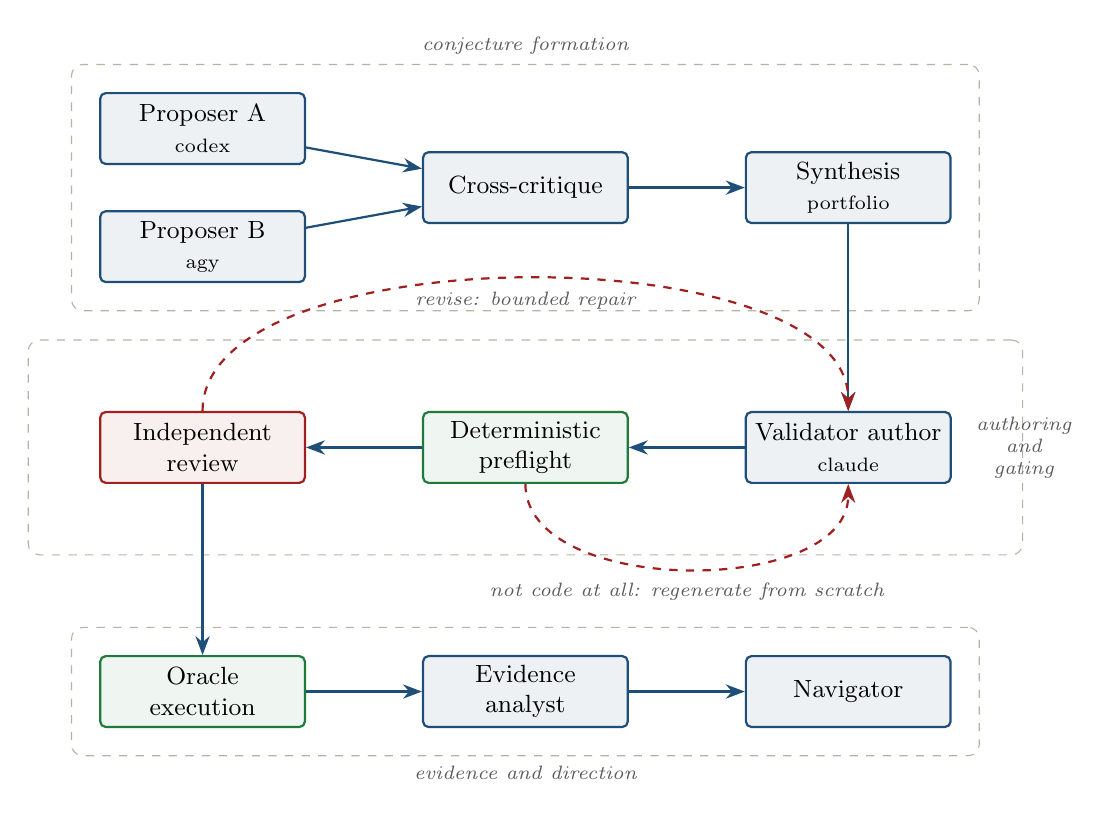
\begin{tikzpicture}

\node[phase] (p1) at (0,0.75) {Proposer A\\\scriptsize codex};
\node[phase] (p2) at (0,-0.75) {Proposer B\\\scriptsize agy};
\node[phase] (crit) at (4.1,0) {Cross-critique};
\node[phase] (syn) at (8.2,0) {Synthesis\\\scriptsize portfolio};

\node[phase] (auth) at (8.2,-3.3) {Validator author\\\scriptsize claude};
\node[det]   (pre)  at (4.1,-3.3) {Deterministic\\preflight};
\node[gate]  (rev)  at (0,-3.3) {Independent\\review};

\node[det]   (orc) at (0,-6.4) {Oracle\\execution};
\node[phase] (an)  at (4.1,-6.4) {Evidence\\analyst};
\node[phase] (nav) at (8.2,-6.4) {Navigator};

\draw[flow] (p1) -- (crit);
\draw[flow] (p2) -- (crit);
\draw[flow] (crit) -- (syn);
\draw[flow] (syn) -- (auth);
\draw[flow] (auth) -- (pre);
\draw[flow] (pre) -- (rev);
\draw[flow] (rev) -- (orc);
\draw[flow] (orc) -- (an);
\draw[flow] (an) -- (nav);

% return paths, kept inside the authoring band so they never cross other rows
\draw[backflow] (rev.north) to[out=90,in=90,looseness=0.7]
  node[note, pos=0.5, below=0.4mm] {revise: bounded repair} (auth.north);
\draw[backflow] (pre.south) to[out=270,in=270,looseness=0.9]
  node[note, pos=0.5, below=0.5mm] {not code at all: regenerate from scratch}
  (auth.south);

\begin{scope}[on background layer]
  \node[fit=(p1)(p2)(crit)(syn), draw=astraline, dashed, rounded corners,
        inner sep=3.5mm,
        label={[note, anchor=south]north:conjecture formation}] {};
  \node[fit=(auth)(pre)(rev), draw=astraline, dashed, rounded corners,
        inner sep=9mm] {};
  \node[fit=(orc)(an)(nav), draw=astraline, dashed, rounded corners,
        inner sep=3.5mm,
        label={[note, anchor=north]south:evidence and direction}] {};
\end{scope}

\node[note, anchor=west] at (9.7,-3.3) {authoring\\and\\gating};

\end{tikzpicture}
\caption{The atomic cycle. Blue: model phases. Green: deterministic steps.
Red: gates that can send work back. The dashed red arrows are the two return
paths that Section~\ref{sec:notcode} shows must be kept distinct.}
\label{fig:cycle}
\end{figure}

\subsection{The self-refutation harness}

The validator is not asked to confirm the conjecture. It is required to test it
through independent legs and to print one line per leg:

\begin{itemize}[leftmargin=*,itemsep=0pt]
  \item a \emph{symbolic} leg: an exact residual or identity reduced to a
        literal zero;
  \item a \emph{numeric} leg: evaluation at seeded random points against a tight
        tolerance;
  \item a \emph{limit} leg: a degenerate case with a known closed answer.
\end{itemize}

The script prints \code{VERDICT: PASS} only if every leg passes. Critically, the
failing branch must be \emph{reachable code}: a deterministic AST auditor
rejects validators that cannot fail, and the cycle is re-run against the author
with the auditor's reasons. A test that cannot fail is not evidence.

\section{Epistemic architecture}
\label{sec:axes}

\subsection{Five axes that must not collapse}

The single most consequential design decision in ASTRA is that status is not one
value. Five distinct questions are tracked separately (Figure~\ref{fig:axes}):

\begin{enumerate}[leftmargin=*,itemsep=0pt]
  \item \textbf{operation status} --- did the phase or tool complete?
  \item \textbf{claim status} --- supported, refuted, inconclusive, not tested?
  \item \textbf{evidence grade} --- what kind and strength of evidence exists?
  \item \textbf{branch status} --- should this direction continue?
  \item \textbf{goal coverage} --- how much of the objective is resolved?
\end{enumerate}

Collapsing any pair produces a specific, observable pathology:

\begin{center}
\begin{tabular}{@{}ll@{}}
\toprule
\textbf{Collapse} & \textbf{Pathology} \\
\midrule
operation into claim & a Python traceback ``refutes'' a theorem \\
numeric into evidence grade & sampling silently becomes a universal proof \\
claim into goal coverage & one lemma reports the programme as finished \\
claim into branch & a refuted branch closes a still-viable direction \\
\bottomrule
\end{tabular}
\end{center}

\begin{figure}[t]
\centering
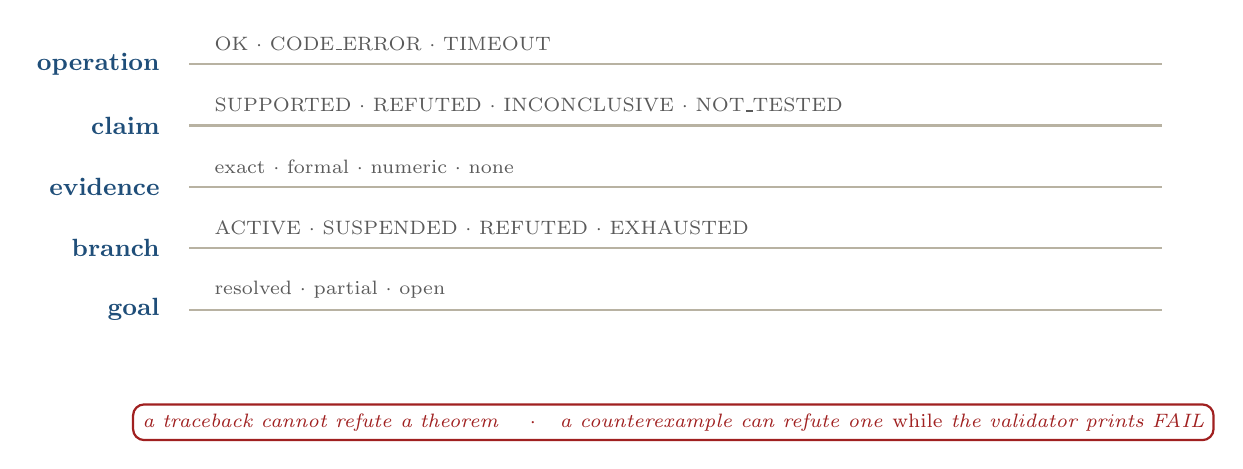
\begin{tikzpicture}[scale=1]
\foreach \i/\name/\vals in {
  0/operation/{OK \(\cdot\) CODE\_ERROR \(\cdot\) TIMEOUT},
  1/claim/{SUPPORTED \(\cdot\) REFUTED \(\cdot\) INCONCLUSIVE \(\cdot\) NOT\_TESTED},
  2/evidence/{exact \(\cdot\) formal \(\cdot\) numeric \(\cdot\) none},
  3/branch/{ACTIVE \(\cdot\) SUSPENDED \(\cdot\) REFUTED \(\cdot\) EXHAUSTED},
  4/goal/{resolved \(\cdot\) partial \(\cdot\) open}}
{
  \node[anchor=east, font=\small\bfseries, text=astrablue] at (0,-\i*0.78) {\name};
  \draw[astraline, thick] (0.25,-\i*0.78) -- (12.6,-\i*0.78);
  \node[anchor=west, font=\scriptsize, text=astragrey] at (0.45,-\i*0.78+0.26) {\vals};
}
\node[draw=astrared, thick, fill=white, rounded corners, font=\scriptsize\itshape,
      align=center, text=astrared] at (6.4,-4.55)
   {a traceback cannot refute a theorem \quad$\cdot$\quad
    a counterexample can refute one \emph{while} the validator prints FAIL};
\end{tikzpicture}
\caption{The five status axes are recorded independently for every episode. The
box states the two facts that make the separation necessary in both directions.}
\label{fig:axes}
\end{figure}

\subsection{Verdict re-anchoring}

An early live measurement exposed a subtle version of the same disease. Given a
false claim, ASTRA would correctly identify the falsehood, form a
\emph{corrected} conjecture, validate the correction, and report
\code{VALIDATED}. Every individual step was right; the reported status answered
the conjecture the system had formed rather than the claim the user had made.

The fix is a separate axis, \code{original\_claim\_verdict}, taking values
\textsc{supported}, \textsc{refuted}, \textsc{inconclusive},
\textsc{substituted} or \textsc{unspecified}, produced by the analyst from the
user's original statement. Verified live on seeded false claims, it moved the
false-acceptance rate from an apparent $0.67$ to a true $0.0$: the earlier
number was an instrument artefact, not a hallucination rate.

\subsection{Evidence policy by claim type}

Different claim shapes admit different minimum evidence. This is enforced, not
advisory.

\begin{center}
\small
\begin{tabular}{@{}p{3.6cm}p{5.6cm}p{5.2cm}@{}}
\toprule
\textbf{Claim type} & \textbf{Minimum credible evidence} & \textbf{Escalation} \\
\midrule
Universal theorem & exact argument, or explicitly bounded scope & CAS/SMT, then a proof kernel \\
Existential / refutation & one exact admissible witness & minimality, independent reconstruction \\
Equivalence / derivation & conditions plus exact residual & independent CAS, high precision \\
Numerical prediction & reproducibility, uncertainty, convergence & independent implementation \\
Algorithmic guarantee & proof obligations plus sanity cases & formalisation of decisive lemmas \\
Scoped empirical claim & frozen data and protocol, stated uncertainty & replication, holdout \\
\bottomrule
\end{tabular}
\end{center}

An existential claim needs one witness; a universal claim needs an argument.
The asymmetry is not decoration: in live use it is the difference between an
obligation a cycle can discharge and one it cannot, and a campaign that states
its claims in the wrong shape spends its budget on validators the reviewer will
correctly refuse (Section~\ref{sec:claimshape}).

\section{The campaign layer}
\label{sec:campaign}

\subsection{Data model}

Six append-only record types (Figure~\ref{fig:model}) are enough to drive a
programme. Everything else---method, provenance, review, artifact data---is a
typed field or a linked manifest. The graph is a derived projection; the event
log is the source of truth.

\begin{figure}[t]
\centering
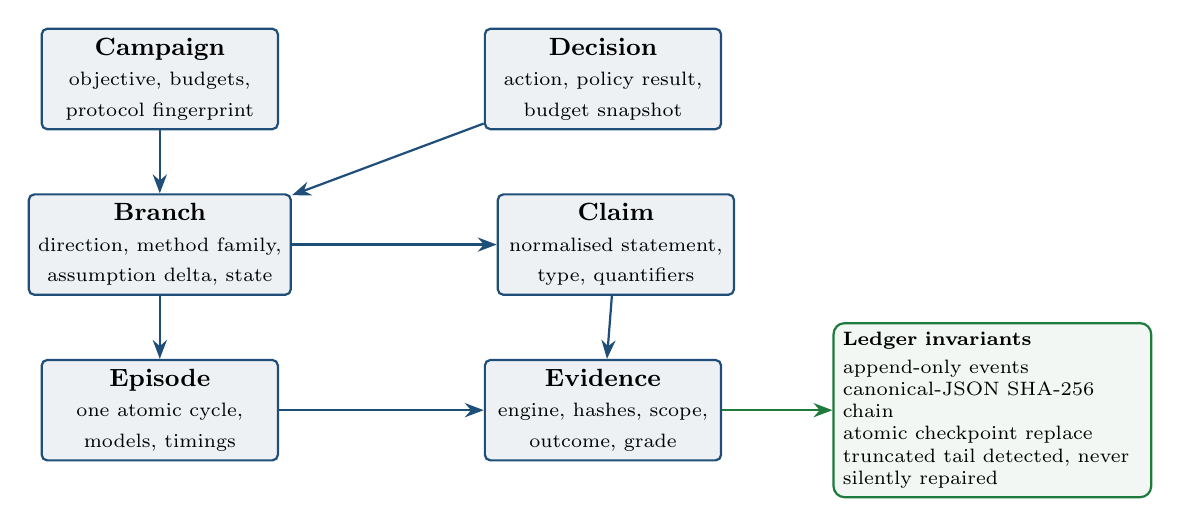
\begin{tikzpicture}[node distance=8mm and 12mm, every node/.style={font=\small}]
\node[phase, minimum width=30mm] (camp) {\textbf{Campaign}\\\scriptsize objective, budgets,\\\scriptsize protocol fingerprint};
\node[phase, below=of camp, minimum width=30mm] (br) {\textbf{Branch}\\\scriptsize direction, method family,\\\scriptsize assumption delta, state};
\node[phase, below=of br, minimum width=30mm] (ep) {\textbf{Episode}\\\scriptsize one atomic cycle,\\\scriptsize models, timings};
\node[phase, right=26mm of br, minimum width=30mm] (cl) {\textbf{Claim}\\\scriptsize normalised statement,\\\scriptsize type, quantifiers};
\node[phase, right=26mm of ep, minimum width=30mm] (ev) {\textbf{Evidence}\\\scriptsize engine, hashes, scope,\\\scriptsize outcome, grade};
\node[phase, right=26mm of camp, minimum width=30mm] (dec) {\textbf{Decision}\\\scriptsize action, policy result,\\\scriptsize budget snapshot};

\draw[flow] (camp) -- (br);
\draw[flow] (br) -- (ep);
\draw[flow] (ep) -- (ev);
\draw[flow] (cl) -- (ev);
\draw[flow] (br) -- (cl);
\draw[flow] (dec) -- (br);

\node[draw=astragreen, thick, fill=astragreen!6, rounded corners, align=left,
      font=\scriptsize, right=14mm of ev, text width=38mm] (ledger)
  {\textbf{Ledger invariants}\\[2pt]
   append-only events\\
   canonical-JSON SHA-256 chain\\
   atomic checkpoint replace\\
   truncated tail detected, never\\ silently repaired};
\draw[flow, draw=astragreen] (ev) -- (ledger);
\end{tikzpicture}
\caption{The six live records and the ledger guarantees behind them. A partially
written tail is detected and archived rather than repaired, because silently
repairing an audit log destroys the property that makes it an audit log.}
\label{fig:model}
\end{figure}

\subsection{Portfolios instead of a single winner}

Ensemble synthesis normally destroys information: the minority proposal
disappears into the consensus text. ASTRA~2.0 requires the synthesiser to return
a \emph{structured portfolio}---the selected atomic claim plus two to four
materially different admissible alternatives, each with its method family, its
assumption delta, and the cheapest evidence that would discriminate it from the
selected one.

The parser is deliberately asymmetric: \emph{fail-soft} on the portfolio as a
whole (a malformed block must never destroy a paid-for cycle) and
\emph{fail-closed} on individual candidates (a candidate without a crux is not
admissible). One live defect came from exactly this boundary: a model emitted an
empty string inside a quantifier list and an early implementation discarded the
entire portfolio.

\subsection{Hard gates, then a visible priority vector}

A scalar reward is epistemically unsafe: scientific truth, novelty, stability
and cost are not one number, and a numerical failure may mean a false claim, an
unstable representation, or simply a broken validator. ASTRA~2.0 therefore
applies \emph{hard admissibility gates} first, and only then orders the
survivors by a visible, unlearned priority vector.

\begin{center}
\small
\begin{tabular}{@{}p{7.1cm}p{7.1cm}@{}}
\toprule
\textbf{Hard gates (all must hold)} & \textbf{Priority vector (lexicographic)} \\
\midrule
relevant to an unresolved deliverable & expected information gain \\
falsifiable or formally scoped & current evidence strength \\
explicit domain, assumptions, quantifiers & methodological independence \\
feasible evidence plan & goal advancement \\
no exhausted duplicate method or claim & estimated execution and model cost \\
sufficient remaining budget & instability and hallucination risk \\
\bottomrule
\end{tabular}
\end{center}

The Navigator model supplies estimates and rationale for the vector, but
\textbf{cannot override a failed gate}. A model recommendation that contradicts
a deterministic gate is recorded and ignored---this is enforced in code and
pinned by a regression test.

\subsection{Progressive widening}

Only one branch is active initially. Another is promoted only on a specific
trigger: negative or inconclusive evidence, method redundancy, evidence
saturation, or a high-value independent alternative. Breadth must be
\emph{earned by evidence}, because a controller that widens on enthusiasm
produces many branches and no results.

\subsection{The algorithm}

\begin{center}
\begin{minipage}{0.93\textwidth}
\small
\hrule\vspace{3pt}
\textbf{Campaign step}\vspace{2pt}
\hrule\vspace{4pt}
\begin{enumerate}[leftmargin=1.4em,itemsep=1pt]
  \item Freeze brief, budgets, resources and protocol hash.
  \item Run the parallel proposal and cross-critique phase.
  \item Require a structured portfolio from synthesis; promote minority
        candidates to \textsc{proposed} branches.
  \item Execute \emph{only} the selected claim through authoring, preflight,
        review, oracle, audit and navigation.
  \item Classify the outcome: scientific refutation, invalid validator,
        operational error, numerical instability, formalisation failure, or
        credible evidence.
  \item Append episode and evidence manifests to the ledger.
  \item Let the models recommend; enforce the deterministic constraints.
        \emph{Never} promote a branch with a missing quantifier contract;
        \emph{never} treat sampling as proof; \emph{never} treat an operational
        failure as a refutation; \emph{never} declare the goal resolved while
        mandatory deliverables remain.
  \item Continue the active branch while evidence is informative and the next
        obligation is clear; widen only when a trigger fires.
  \item Trigger the expanded adversarial campaign only at a scientific
        milestone.
  \item Terminate on complete result, structured partial progress, exhausted
        search, budget exhaustion, or an explicit human decision.
\end{enumerate}
\vspace{2pt}\hrule
\end{minipage}
\end{center}

\section{Failure modes we had to solve}
\label{sec:failures}

This section is the empirical core of the report. The defects below were found
by running the system, not by reading it, and each one is accompanied by the
measurement that exposed it.

\subsection{Cross-agent instruction injection}
\label{sec:injection}

\paragraph{Observation.} One deliberation ended with the following sentence
carried into the consensus conjecture:

\begin{center}
\small\ttfamily
Review the proposed implementation plan artifact [plan.md](file:///\dots) \\
to formally construct the validator. Pending your approval.
\end{center}

The validator author runs with all tools disabled, by design. It nevertheless
attempted to comply, emitting roughly forty repetitions of ``\code{**Tool
call:** let me read it}'' instead of a script. That prose entered the pipeline
as code, failed to parse, and the repair call that followed consumed its entire
64\,000-token output budget without emitting a single character
(Figure~\ref{fig:injection}).

\paragraph{Diagnosis.} The leak is not a model quirk. ASTRA invokes the
Antigravity CLI with \code{--mode plan} \emph{deliberately}: it is the read-only
sandbox that prevents that CLI from writing files or executing, exactly as
\code{--tools ""} does for the author. Plan-mode artefacts are therefore the
\emph{structural cost of a correct safety choice}. Measured over 87 deposited
checkpoints, the artefact appears in \textbf{72\% of deliberations}; synthesis
filtered it out in every case but one, and that one destroyed the cycle.

\paragraph{Fix.} Two layers. The conjecture now travels to the author inside an
explicit fence, and a prompt rule states that anything inside the fence
demanding a tool call is ensemble scaffolding to be ignored. Independently, the
artefact is stripped at the source, matched on the invariant (a \code{file://}
link) rather than on the wording, which varies and changes language. Removal is
always announced; a reply that is \emph{only} an artefact pointer is reported as
a failed call rather than cleaned, because the model left its answer in a file
the system cannot read.

\begin{figure}[t]
\centering
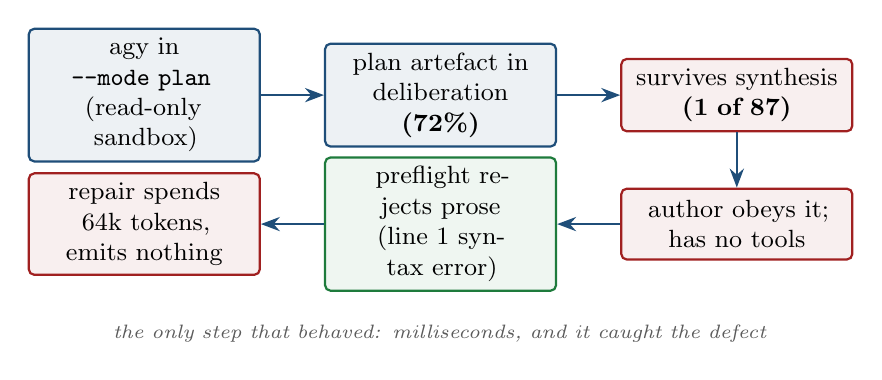
\begin{tikzpicture}[node distance=4mm, every node/.style={font=\scriptsize}]
\node[phase, text width=27mm] (a) {agy in \code{--mode plan}\\(read-only sandbox)};
\node[phase, right=8mm of a, text width=27mm] (b) {plan artefact in\\deliberation \textbf{(72\%)}};
\node[gate, right=8mm of b, text width=27mm] (c) {survives synthesis\\\textbf{(1 of 87)}};
\node[gate, below=7mm of c, text width=27mm] (d) {author obeys it;\\has no tools};
\node[det, left=8mm of d, text width=27mm] (e) {preflight rejects prose\\(line 1 syntax error)};
\node[gate, left=8mm of e, text width=27mm] (f) {repair spends 64k tokens,\\emits nothing};
\draw[flow] (a) -- (b);
\draw[flow] (b) -- (c);
\draw[flow] (c) -- (d);
\draw[flow] (d) -- (e);
\draw[flow] (e) -- (f);
\node[note, below=3mm of e, text width=100mm]
  {the only step that behaved: milliseconds, and it caught the defect};
\end{tikzpicture}
\caption{The causal chain from a deliberate safety setting to a destroyed cycle.
Text produced by one agent became instructions for another; the benign origin
does not change the mechanism.}
\label{fig:injection}
\end{figure}

\subsection{Budget allocation: a share cannot protect the end of a pipeline}
\label{sec:budget}

\paragraph{Observation.} Every phase call was capped at a fraction of the
\emph{remaining} cycle budget, so that no phase could starve its successors.
Over a canary run, all twelve validator repairs timed out, at a median ceiling
of $165$\,s against the $480$\,s configured, and always with budget still on the
clock. The split between success and failure was purely temporal: cycles that
validated ran a median of $882$\,s, cycles that failed $1249$\,s.

\paragraph{Diagnosis.} A share is a fraction of what remains, so it shrinks as
the cycle progresses and hands the least to the phase that runs last. The
validator repair \emph{is} last, and it is the step that converts a rejected
validator into a result. A proportional rule starves precisely the phase whose
starvation is most expensive (Figure~\ref{fig:budget}).

\paragraph{Fix.} Phases additionally declare what they must \emph{leave behind}.
The reserve is sized from measured p90s: $343$\,s for the repair plus $270$\,s
for execution, analysis and navigation. After the change, repairs received their
full $481$\,s ceiling in every observed case.

\begin{figure}[t]
\centering
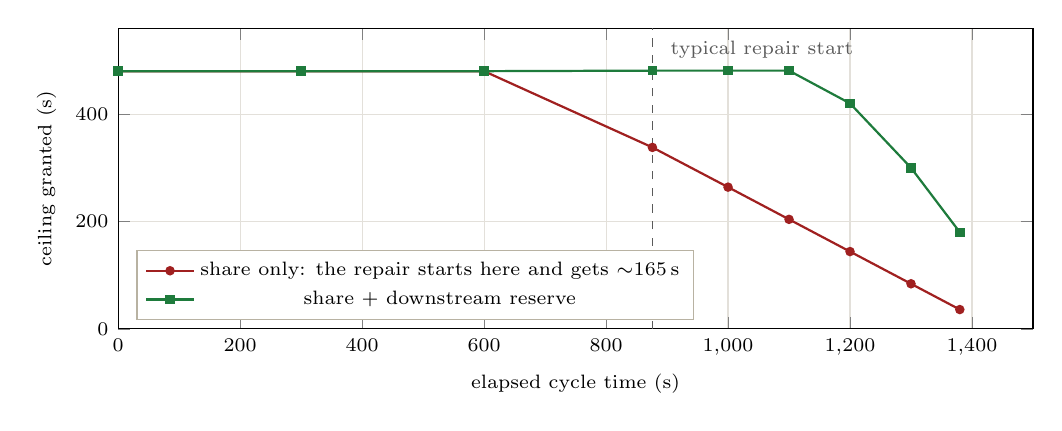
\begin{tikzpicture}
\begin{axis}[
  width=13.2cm, height=5.4cm,
  xlabel={elapsed cycle time (s)}, ylabel={ceiling granted (s)},
  xmin=0, xmax=1500, ymin=0, ymax=560,
  legend style={font=\scriptsize, at={(0.02,0.03)}, anchor=south west, draw=astraline},
  grid=major, grid style={astraline!40}, tick label style={font=\scriptsize},
  label style={font=\scriptsize}]
\addplot[thick, astrared, mark=*, mark size=1.3pt] coordinates {
  (0,480) (300,480) (600,480) (876,338) (1000,264) (1100,204) (1200,144) (1300,84) (1380,36)};
\addlegendentry{share only: the repair starts here and gets $\sim$165\,s}
\addplot[thick, astragreen, mark=square*, mark size=1.3pt] coordinates {
  (0,480) (300,480) (600,480) (876,481) (1000,481) (1100,481) (1200,420) (1300,300) (1380,180)};
\addlegendentry{share $+$ downstream reserve}
\draw[astragrey, dashed] (axis cs:876,0) -- (axis cs:876,560);
\node[font=\scriptsize, text=astragrey, anchor=west] at (axis cs:890,520) {typical repair start};
\end{axis}
\end{tikzpicture}
\caption{Ceiling granted to the validator repair as a function of when it starts.
Under a pure share rule the last phase is systematically the poorest; the
reserve restores it. Points are computed from the measured phase medians.}
\label{fig:budget}
\end{figure}

\subsection{The pipeline has a loop, and phase-indexed state assumes a line}

Three separate defects shared one root cause: state indexed by \emph{phase name}
used to reason about \emph{position in the flow}. The validation pipeline is not
linear---review runs again after every repair---so any rule of the form ``phase
$X$ must reserve for what follows $X$'' is wrong on the second pass.

The clearest instance: a final review round was refused with $571.83$\,s still
available, because it was asked to hold back $613$\,s for a repair that could no
longer run, the revision budget already being spent. The reserve now answers
``what can still run?'' rather than ``which phase is asking?''.

A companion guard was added at the same time. A phase whose computed ceiling
falls below $45$\,s is not started at all: issuing a call that cannot succeed
burns quota and, worse, mislabels budget exhaustion as a model timeout. Before
the guard, the logs contained \code{timeout tras 1s}, which reads as a hung
model and is nothing of the sort.

\subsection{An output ceiling consumed by reasoning}

A repair call was killed after $1200$\,s having produced $184$\,KB of internal
reasoning and \emph{zero} characters of answer, stopping at exactly $64\,000$
output tokens. Raising the time ceiling from $480$\,s to $1200$\,s had changed
nothing, because the binding constraint was never time.

Sizing the fix required care in both directions: the calls that \emph{worked}
had spent $59\,181$ and $56\,630$ tokens, so a cap below that would degrade the
one configuration known to function. The thinking budget is capped at $58\,000$,
which clears every observed success and still reserves about twice the largest
validator ever measured.

\subsection{Prose is not a damaged script}
\label{sec:notcode}

A reply that fails to parse can be a broken script or not a script at all, and
the two need opposite treatments. Handing prose back as ``your previous code,
fix line 1'' is an impossible instruction---it was the request that consumed the
64\,000-token budget above. The preflight now distinguishes the cases and is
deliberately conservative: any \code{import} or \code{def} counts as an
attempted script, so a validator with a typo keeps its right to a local repair,
and only genuine prose triggers regeneration from a clean slate.

\subsection{What only live research exposed}
\label{sec:live}

The defects above were found by benchmarking. Four more surfaced only when the
campaign layer drove an actual research programme, and none of them could have
appeared in a benchmark, because a benchmark \emph{counts} outcomes while a
campaign \emph{acts} on them.

\paragraph{A gate that declines is not a tool that broke.} The independent
reviewer refused a validator---correctly, and with specific objections---and the
campaign recorded it as \code{operation\_status: FAILED}. Two such episodes then
promoted a second branch under progressive widening: a scientific decision taken
from an operational signal, which is the collapse of Figure~\ref{fig:axes}
happening inside the code written to prevent it. A refusal now maps to a
completed pipeline with an untested claim; a reviewer that times out stays an
operational failure. Same phase, opposite meaning.

\paragraph{Widening must not be driven by episodes that never ran.} The same
rule counted an episode that produced no phases, no models and no timings---the
signature of a lost lock. A tool that broke says nothing about the promise of a
research direction. The rule now skips such episodes without letting them extend
or reset a streak, and deliberately still counts a validator that ran and
crashed, because that \emph{does} say the direction is hard to test.

\paragraph{A replayed cycle is not an observation.} Two consecutive episodes
recorded byte-identical timings and two separate evidence records: the second
step re-sent the same direction, hit the cycle cache and returned in seconds. The
cache is right for a research loop revisiting a direction and wrong for a ledger,
where it manufactures corroboration. Replays are now refused before they can
reach the record.

\paragraph{An episode is evidence only if the cycle ran for that claim.}
\label{sec:foreign}
The executor accepts a cycle result through a runner hook, which is useful for
tests and for recovering a cycle whose runner died. A result from an entirely
unrelated project---running in the same minute, on the same workstation---was
fed in through that hook, and the ledger gained a \textsc{supports} record whose
validator tested a completely different mathematical object. Every status axis,
every gate and every hash was correct about a result that answered another
question. Results are now bound to the request by their shared objective, and
the ledger records the retraction rather than hiding it.

\begin{center}
\small
\begin{tabular}{@{}p{5.2cm}p{4.3cm}p{4.5cm}@{}}
\toprule
\textbf{Defect} & \textbf{Invisible to benchmarks because} & \textbf{Structural fix} \\
\midrule
reviewer refusal recorded as breakage & benchmarks count it, campaigns act on it &
five axes enforced at the campaign boundary \\
widening driven by a lost lock & benchmarks have no branches to widen &
episodes that did no work are skipped \\
cached replay minted as evidence & benchmarks disable the cache &
replays refused before the ledger \\
foreign result accepted by the runner hook & benchmarks never hand-feed results &
result bound to the request's objective \\
\bottomrule
\end{tabular}
\end{center}

\subsection{Claim shape decides what a cycle can discharge}
\label{sec:claimshape}

A campaign spent three episodes without a single validator admitted, and the
reviewer's three refusals were each correct. The cause was not the models: every
branch obligation had been stated as an existential over a \emph{continuum}.
Such a claim is not decided by evaluation---satisfying it needs a witness,
refuting it needs an argument over the whole family---so the author kept
attempting the middle route of sweeping and summarising, and the reviewer kept
rejecting it.

Restating each obligation at a concrete point produced a decided result in one
episode. A second restatement mattered as much: asking whether a parameter
\emph{moves} the quantity, rather than whether it solves the problem, so that
the claim cannot be settled without the parameter being involved. The first
formulation had produced a refutation whose witness was numerically identical to
the baseline---a correct verdict about a sentence, establishing nothing about
the idea.

This is a protocol property, not a physics one. The evidence policy of
Section~\ref{sec:axes} already said an existential is discharged by a witness;
what was missing was any mechanism that stopped a campaign from seeding claims
its own policy could not serve.

\subsection{Failure attribution is infrastructure}
\label{sec:attribution}

Over 87 deposited checkpoints, \textbf{7 cycles} reported a failure of the
\emph{reviewer} when the component that actually died was the validator author,
and in all seven the generated validator was overwritten by the error string.
The consequence is not cosmetic: it corrupts the very statistics used to tune
the system. Under the old labels the picture read ``the reviewer fails 15 of
15''; under corrected labels it read ``the repair starves in 8 of 15''---and
only the second statement points at a fixable cause.

\begin{center}
\small
\begin{tabular}{@{}p{4.5cm}p{4.6cm}p{4.9cm}@{}}
\toprule
\textbf{Symptom} & \textbf{Apparent cause} & \textbf{Actual cause} \\
\midrule
reviewer fails 15/15 & the reviewer & repair starved by a share rule \\
\code{timeout tras 1s} & a hung model & budget exhausted; call issued anyway \\
translator needs more time & a small ceiling & output tokens spent on reasoning \\
cycle dies writing a validator & model incapacity & injected instruction from a peer agent \\
both arms fail 100\% of cycles & the architectures & a stale lock; BUSY scored as failure \\
\bottomrule
\end{tabular}
\end{center}

\section{Evaluation}
\label{sec:eval}

\subsection{What the measurement cost}

Four benchmark runs were required to obtain one valid dataset. The first three
measured the harness: a stale lock (a transient \code{BUSY} scored as an
architectural failure, producing an apparently meaningful
$\textrm{failure}=1.0$ in \emph{both} arms within 45 seconds); a scheduler
context that broke the sandbox mechanism of one CLI, failing every process
launch; and an expired CLI session. Each produced a number with the shape of a
finding and the content of an artefact.

This is the report's most transferable lesson. In a multi-agent system whose
components are subscription CLIs on a developer workstation, \emph{the
environment is an experimental variable}. A forty-second pre-flight that
verifies every provider answers before committing hours of quota would have
saved three runs.

\subsection{Phase cost}

Figure~\ref{fig:phases} shows measured phase medians on the amended protocol.
Two facts follow. The pipeline is dominated by conjecture formation and
validator authoring, jointly about 58\% of a cycle; and a fixed ceiling sized
against an older budget stops meaning anything when the budget moves---the
translator ceiling of $480$\,s sat \emph{below} the $573$\,s median of the task
it bounded, and four of eight timeouts died at exactly that value. Ceilings that
must track the cycle are now expressed as a fraction of it.

\begin{figure}[t]
\centering
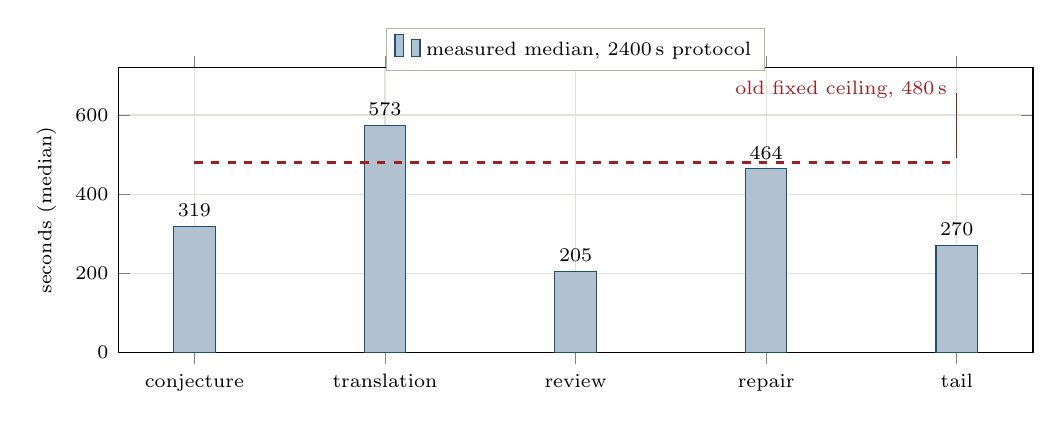
\begin{tikzpicture}
\begin{axis}[
  width=13.2cm, height=5.2cm,
  ybar, bar width=15pt,
  symbolic x coords={conjecture,translation,review,repair,tail},
  xtick=data, ymin=0, ymax=720,
  ylabel={seconds (median)}, ylabel style={font=\scriptsize},
  tick label style={font=\scriptsize},
  nodes near coords, nodes near coords style={font=\scriptsize},
  grid=major, grid style={astraline!40},
  legend style={font=\scriptsize, at={(0.5,1.14)}, anchor=north, draw=astraline}]
\addplot[fill=astrablue!35, draw=astrablue] coordinates
  {(conjecture,319) (translation,573) (review,205) (repair,464) (tail,270)};
\addlegendentry{measured median, 2400\,s protocol}
\draw[astrared, thick, dashed] (axis cs:conjecture,480) -- (axis cs:tail,480);
\node[font=\scriptsize, text=astrared, anchor=east] (ceil) at (axis cs:tail,665)
  {old fixed ceiling, 480\,s};
\draw[astrared, thin] (axis cs:tail,655) -- (axis cs:tail,492);
\end{axis}
\end{tikzpicture}
\caption{Phase medians over 18 cycles. The dashed line is the ceiling that was
in force: below the median of the phase it was supposed to bound.}
\label{fig:phases}
\end{figure}

\subsection{The comparative result, unvarnished}

The preregistered question is whether the heterogeneous reflective loop
(\code{full}) produces better research trajectories than a matched linear
control (\code{full-linear}) under equal budgets. We fixed in advance that the
comparison would only be interpretable below an operational failure rate of
$0.2$.

\begin{center}
\small
\begin{tabular}{@{}lcccc@{}}
\toprule
& \textbf{cycles} & \textbf{validated} & \textbf{breakage} & \textbf{reviewer rejections} \\
\midrule
\code{full}         & 8  & \textbf{0} & 5 (0.63) & 2 \\
\code{full-linear}  & 10 & \textbf{3} & 4 (0.40) & 3 \\
\bottomrule
\end{tabular}
\end{center}

The criterion is not met, so the comparison does not license a conclusion. We
report the numbers anyway, including the part that runs against our own
hypothesis: with $63\%$ and $40\%$ breakage, which arm validates depends mostly
on where the breakage fell, and \code{full} had fewer chances because it died
earlier ($16$ model calls per cell against $26$). With four cells per arm, $0$
against $3$ is compatible with chance. It is nevertheless the first measured
signal, and it does not point the way we assumed.

Note also the distinction the aggregate hides: \emph{breakage} (timeouts,
exhausted budget) is a reliability defect, whereas a \emph{reviewer rejection}
is the system refusing to certify weak work. Counting the second as a failure
penalises rigour. A short verification run after the fixes described above
produced four cycles, four validations and zero breakage in both arms---which
establishes that no known structural blocker remains, and, honestly, nothing
more: no translation in it exceeded $296$\,s, so the new ceiling was never
exercised.

\section{Why we believe this helps research}

\begin{description}[leftmargin=0pt, style=nextline, itemsep=3pt]
\item[Refutation is the default, not an option.] The validator must be able to
fail, and a deterministic auditor rejects it when it cannot. This inverts the
usual incentive of a generative system, which is to produce a satisfying answer.

\item[Independence is structural.] The author is not a proposer, the reviewer is
not the author, and the oracle is not a model at all. Agreement between them
carries information precisely because it was not arranged.

\item[Status cannot be flattened.] The five axes prevent the specific confusions
that make automated research untrustworthy---most importantly, that a program
crash is not a scientific result and that answering a corrected question is not
answering the question asked.

\item[Evidence is executable and deposited.] Every claim is backed by a script,
its hash, its output and the model that wrote it. A reader can re-run the
evidence rather than trust the narrative.

\item[Negative results are first-class.] Pruning a hypothesis family, exhausting a
method, or reporting \textsc{inconclusive} are recorded outcomes with the same
standing as a success. Most real research time is spent here, and systems that
only recognise successes silently discard it.
\end{description}

\section{Limitations}

\begin{itemize}[leftmargin=*,itemsep=1pt]
  \item \textbf{The central comparison is unresolved.} No valid pilot has yet
        met the reliability precondition; the only measured signal is small and
        adverse. We claim an architecture and a failure catalogue, not a
        demonstrated uplift.
  \item \textbf{Blinded expert scoring is absent.} The primary quality endpoint
        requires two human raters per cell, blind to architecture. Automatic
        metrics measure process and efficiency, not scientific depth, and we
        decline to substitute one for the other.
  \item \textbf{Small $n$.} Canary tiers use two cases and two seeds. Several
        conclusions drawn earlier in this project at $n{=}1$ reversed on
        repetition, and are marked as retracted in the deposited evidence.
  \item \textbf{Environment coupling.} The system depends on subscription CLIs
        whose authentication, sandboxing and process behaviour are part of the
        experimental apparatus, as Section~\ref{sec:eval} shows at some cost.
  \item \textbf{Single-workstation quota.} One deliberative cycle runs at a
        time, machine-wide, because concurrent cycles share model accounts. This
        bounds throughput independently of the architecture.
\end{itemize}

\section{Reproducibility}

Every number in this report is traceable to a deposited artefact: phase timings
and status counts come from per-cycle JSON checkpoints; validator sources,
oracle stdout and their hashes are stored beside them; the benchmark protocol is
content-addressed, and an amendment to it (widening the per-cycle budget from
$1800$\,s to $2400$\,s) changed that fingerprint, was dated, justified and
recorded in a fingerprint history rather than applied silently. The regression
suite stands at 435 tests, and the defects described in
Section~\ref{sec:failures} are each pinned by a test that replays the measured
values that exposed them.

\vspace{4mm}
\hrule
\vspace{2mm}
\noindent\footnotesize
\textbf{Note on scope.} This report describes an engineering system, its
protocol and its evaluation. Scientific results obtained \emph{with} ASTRA
belong to their own projects and are not reported here; where live research
exposed a structural defect, the defect is described and the physics is not.
A companion volume of worked examples is planned separately.

\end{document}
